\documentclass[11pt]{article}
%\usepackage[utf8]{inputenc}
\usepackage{deauthor,times,graphicx}
%\usepackage{hyperref}
\usepackage{xspace}
\usepackage{xcolor}

\newcommand{\etal}{\textit{et~al.}\xspace}
\newcommand{\eg}{\textit{e.g.}\xspace}
\newcommand{\ie}{\textit{i.e.}\xspace}
\newcommand{\aka}{\textit{a.k.a.}\xspace}
\newcommand{\etc}{etc.\xspace}
\newcommand{\cf}{cf.\/~}
\newcommand\figref[1]{Figure~\ref{#1}}
\newcommand\algref[1]{Algorithm~\ref{#1}}
\newcommand\tabref[1]{Table~\ref{#1}}
\newcommand\secref[1]{Section~\ref{#1}}
\newcommand\equref[1]{Equation~(\ref{#1})}
\newcommand{\fakeparagraph}[1]{\vspace{1mm}\noindent\textbf{#1.}}

\graphicspath{{authorname/}}

\ifodd 1
\newcommand{\rev}[1]{{\color{blue}#1}} %revise of the text
\newcommand{\TODO}[1]{{\textbf{TODO}:{ #1} }}
\newcommand{\zeng}[1]{{\color{brown}#1}} %revise of the text
\else
\newcommand{\rev}[1]{#1}
\newcommand{\TODO}[1]{}
\newcommand{\zeng}[1]{#1}
\fi

\begin{document}

\title{Interaction Management in Crowdsourcing}
\author{author}

\author{
		Yansheng Wang{\small $~^{\dagger}$},
		Tianshu Song{\small $~^{\dagger}$},
		Qian Tao{\small $~^{\dagger}$},
		Yuxiang Zeng{\small $~^{\ddagger}$},
		Zimu Zhou{\small $~^{\#}$}, \\
		Yi Xu{\small $~^{\dagger}$},
		Yongxin Tong{\small $~^{\dagger}$},
		Lei Chen{\small $~^{\ddagger}$} \\
	$~^{\dagger}$BDBC, SKLSDE Lab and IRI, Beihang University, China\\
		$~^{\ddagger}$The Hong Kong University of Science and Technology, Hong Kong SAR, China\\
		$~^{\#}$ Singapore Management University, Singapore\\
		$~^{\dagger}$\{arthur\_wang, songts, qiantao, xuy, yxtong\}@buaa.edu.cn \\
		$~^{\ddagger}$\{yzengal, leichen\}@cse.ust.hk,
		$~^{\#}$zimuzhou@smu.edu.sg
}

\maketitle

\begin{abstract}
Crowdsourcing is anticipated as a promising paradigm for Future of Work (FoW), where groups of humans are engaged for problem-solving, services and innovation which are usually difficult for machines.
During the entire workflow of crowdsourcing, intensive interactions take place between workers and the crowdsourcing platform, as well as among groups of workers. 
For sustainable crowdsourcing, the design and management of these interactions should not regard human workers as machines, but rather as individuals and social beings. 
In this article, we highlight the critical interactions in typical crowdsourcing ecosystems, summarize past efforts on human-centric interaction management in crowdsourcing, and discuss emerging interaction management research towards cross-platform crowdsourcing.
\end{abstract}

% Crowdsourcing, as an effective paradigm to combine the ability of human and machines, has been wildly used in many areas and achieved big success.
% However, existing works mainly model human workers as machines to optimize the performance of crowdsourcing platforms.
% The will of human workers is often ignored, which is a pity.
% We expect that crowdsourcing could provide jobs which can be viewed as the future of the work, where crowd workers are viewed as fully human and their ability can be given fully play and can improved gradually.
% To do so, manage the interactions involving crowd workers in the workflow of crowdsourcing is important.
% In this paper, by analyzing the interactions of crowdsourcing, we first focus on the interaction between the workers and the platforms, and the interaction among workers.
% By review related works, we identify the factors which could be improved.
% We finally discuss the future direct of managing the interaction between different crowdsourcing platforms.
% We hope this paper can bring to the forefront the study on human-centered interaction management in crowdsourcing.
    


\section{Introduction}
Some computation tasks are intractable for computers (or machines) but easy for human beings, such as image recognition, text translation, entity resolution, \etc
Although the new breakthroughs of artificial intelligence and machine learning in recent years have relieved the difficulty of solving computer-hard problems to some degree, it still relies on large scale of training data which needs to be labeled manually.
Crowdsourcing is a calculation paradigm to solve computer-hard tasks effectively and efficiently.
It organizes large scale of human beings as workers through the Internet to solve problems.
For decades, crowdsourcing has been applied in various areas.
Many crowdsourcing platforms have achieved business success.
A typical example is Amazon Mechanical Turk (AMT)~, which is the biggest general-purpose crowdsourcing platform.
According to a blog published by AMT~, in a typical week there are millions of tasks that are processed by over a million workers all over the world.
With the aid of the productive forces of AMT, the famous data set of image recognition, ImageNet~, is labeled and has a huge impact.
Besides, there are many people making a living on the income earned from AMT.

Despite the above achievements of crowdsourcing, the welfare of crowd workers is often neglected.
The workers are usually regraded more as machines with some kinds of computing functions, which seems not a wise choice.
% The tasks assigned to them are often mechanical and boring which 
% ability of workers does not come into play enough.
On the one hand, although workers are viewed as machine, they are not as reliable or stable as computers.
Thus, much effort has to be put to tame the uncertainty of workers by modeling their accuracy rates and aggregating feedbacks.
%~\cite{DBLP:conf/sigmod/GuoPG12,DBLP:journals/pvldb/ZhangCJC13,DBLP:journals/pvldb/CaoSTC12}.
On the other hand, workers are more flexible and intelligent than machines.
If their initiative can be stimulated, crowdsourcing platforms will be more productive and workers' welfare can also be enhanced.

% 	Currently, workers
% 	One the one hand, human beings are not as reliable or stable as machines. 
% 	Thus, many studies~\cite{a,b,c} focus on how to 
% 	One the other hand, compared with machines human beings have subjective initiative which is far from being stimulated and utilized well.
% 	In other words, workers of crowdsourcing should have played a more important role.

To achieve the goals of stimulating the initiative of workers to further improve the effectiveness of crowdsourcing platforms and helping the workers achieve self-actualization to make crowdsourcing a form of the future of work, this paper targets at the optimization of critical interactions in typical crowdsourcing ecosystems.
To optimize the interaction between human workers and the platforms, \ie the human-platform interaction, the \textit{freewill} of human beings should be considered.
The main part of human-platform interaction is task assignment, which assigns crowd tasks to suitable workers.
Most existing studies on task assignment only consider how to maximize the utility and ignore whether the workers would like to perform the assigned tasks.
To make task assignment more humanized, tasks should be assigned to workers based on the workers' will.
More friendly methods of task assignment should be designed.
% 	The key of interaction management is social processes.
% 	Specifically, we need to design interaction methods based on the sociality of human beings.
% 	on all the parts involving workers in the workflow.
% Human workers have two characters.
% First, human beings have freewill.
% We cannot assign tasks to human workers roughly without considering their will.
To optimize the interaction between human workers, \ie the human-human interaction, the \textit{sociality} and \textit{selfishness} of human beings should be considered.
When the tasks are simple or well-paid, workers may complete them more efficiently.
Thus, incentive mechanisms should be designed based on workers' rationality and selfishness.
When the tasks are complex and hard to complete, the platforms need the workers to corporate with each other.
Thus, the social relationships of workers should be considered too.
% to form teams.
% For complex tasks, workers need to corporate.
% When they complete, incentive mechanism should be designed to 
% When they corporate, the social relationships of workers should be considered.
% Second, human beings have selfishness.
% Thus, they need to be motivated to perform tasks.
% Incentive mechanism in crowdsourcing is the main interaction between the workers, which can be divided into collaborative incentive mechanism and competitive incentive mechanism.

The rest of the paper is organized as follows.
We categorize the interactions on crowdsourcing platforms in Sec. 2.
We discuss how to optimize the human-platform interaction and human-human interaction in crowdsourcing in Sec. 3 and Sec. 4 respectively.
We envision the future directions in Sec. 5 and conclude the paper in Sec. 6.

\section{Types of Interactions in Crowdsourcing}

\begin{figure}
\centering
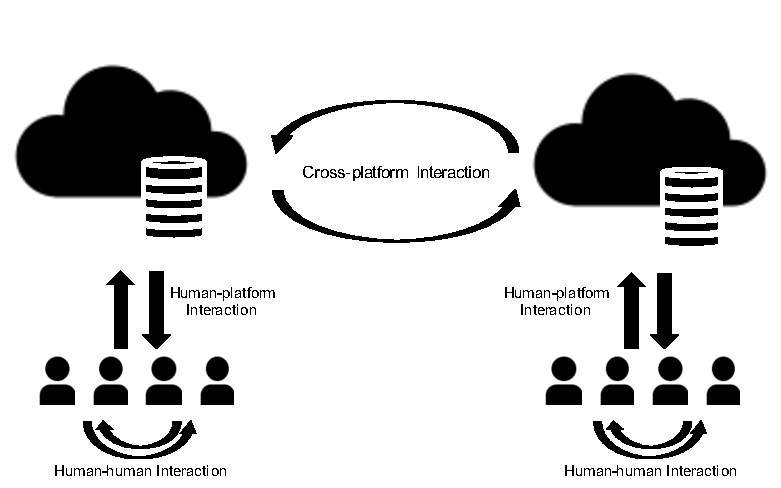
\includegraphics[scale=0.9]{submissions/yongxin/figs/category.pdf}

\caption{Categories of interactions.}
\label{fig:category}
\end{figure}

An interaction process usually involves human workers and platforms as necessary participants. 
Therefore, we can divide interactions on crowdsourcing platforms into three categories: human-platform interaction, human-human interaction and cross-platform interaction, as shown in \figref{fig:category}.

\fakeparagraph{Human-platform interaction}
Interaction between human workers and platforms is an essential process for accomplishing crowdsourced tasks. 
Most human-platform interactive behaviors happen in the task assignment stage, where the platform assigns tasks to appropriate human workers in order to achieve some specific targets such as maximizing the total profits. 
We have recognized that assigning tasks to human workers is rather different from assigning tasks to robots or AI agents, because human workers have free wills and they have rights to reject the assigned tasks or to choose whatever tasks they would like to carry out. 
Therefore, we will focus on the following two kinds of interactions during task assignment process. 
The first is called \textit{task selection by workers}, where the platform displays all available tasks with their specifications, constraints and payments, and the workers can choose the expected tasks freely. This scenario is more common and can be found on many existing crowdsourcing platforms like Amazon Mechanical Turk (AMT) and Figure Eight. 
The second is called \textit{task recommendation by platforms}, where the platform recommends tasks to workers actively and each worker can reject the assignment in which case the platform has to continuously recommend new tasks to them until the task is accepted. 
We will give a detailed introduction to them in Sec. 3.

\fakeparagraph{Human-human interaction}
Apart from the communication between human workers and platforms, there also exist interactions between different workers due to their social activities, which can influence the process of performing the tasks. 
For example, workers with close social relationships like friends or relatives can work together as a team to accomplish complicated tasks.
Considering that human workers are rational and selfish, the platform cannot always expect them to stick together for the sake of finishing all the tasks more effectively and efficiently.
Therefore, proper guidance of human-human interaction like incentive mechanisms can help improve the overall utility meanwhile respecting each individual's interests.
In a way, we can encourage workers to form groups based on their social relations, common likes and dislikes.
They will have \textit{collaborative interaction} between each other, which can be more efficient than working alone.
In another way, we can also allow friendly competitions between workers or groups and give the winners additional rewards.
The \textit{competitive interaction} can improve the efficiency of both sides and can also help the human workers find the value and fun in their efforts.
We will introduce the above two human-human interactions in Sec. 4. 

\fakeparagraph{Cross-platform interaction}
So far, we have discussed about the interactions inside the cycle of a single crowdsourcing platform and its workers. 
But we can also imagine a new type of interaction that exists between different platforms, which we call cross-platform interaction.
Even though today's crowdsourcing platforms are isolated from each other, it is prospective that they cooperate with each other as a federation in the future to serve more tasks and give opportunities to more human workers.
In such a scenario, the cross-platform interaction will play a rather important role.
The challenges of designing proper cross-platform interaction methodology not only lie in dealing with heterogeneous systems, but also in taking care of the unique requirements of human workers: the \textit{privacy concerns}. 
For example, suppose there is a supply constraint on Figure Eight and many tasks on the platform cannot be finished in time. Therefore, Figure Eight wants to federate with AMT which has sufficient worker supply. 
But workers on AMT do not always like to share their profiles and working histories with Figure Eight, which can influence the utility of assignment.  
The two platforms have to interact with each other to form a federation meanwhile no privacy leakage of workers will happen during the interaction process.
We will discuss about such cross-platform interaction as future directions in Sec. 5.

\section{Human-Platform Interaction: Task Assignment} % 3 page
In this section, we focus on the interaction management in task assignment between human workers and platforms.
Specifically, we identify two types of human-platform interactions during the task assignment in crowdsourcing.
In \secref{sec:ta-selection}, we introduce the first type, \ie \textit{task selection by human workers},
where the workers can freely choose the desired tasks 
and a task is assigned to the first worker who selects it.
In \secref{sec:ta-recommend}, we discuss the second type,
\ie \textit{task recommendation by platforms}.
In this type, the platform learns the preferences and profiles of the workers from the history records
and then recommends the suitable tasks to the workers based on different methods.
After that, the human workers can either accept the tasks or reject the tasks.
% Finally, we intrdouce \textit{task bidding between human workers and platforms} in \secref{sec:ta-bidding}.
% In the last type, the procedure of task assignment is usually conducted by auction,
% where the human workers first bid their desired tasks
% and the platform finally decides which of these tasks are allocates to the workers.

\subsection{Task Selection By Human Workers}\label{sec:ta-selection}

In the process of task assignment,
many crowdsourcing platforms apply the strategy of \textit{task selection by human workers} in the interaction management,
\eg Amazon Mechanical Turk, Wikipedia, Quora, Yahoo!Answer.
Specifically, these platforms usually first collect the tasks from the requesters,
then decompose them into micro-tasks~\cite{DBLP:journals/tkde/TongCZJSL18},
and finally pack several micro-tasks into an HIT~(\aka task bin~\cite{DBLP:journals/tkde/TongCZJSL18}).
After the platforms release these HITs into well-designed user interface,
human workers start to interact with the platforms in the process of task assignment.
As shown in \figref{fig:ts-flow}, there are mainly two stages in this workflow: \textit{task selection} and \textit{truth inference}.

\begin{figure}
	\centering
	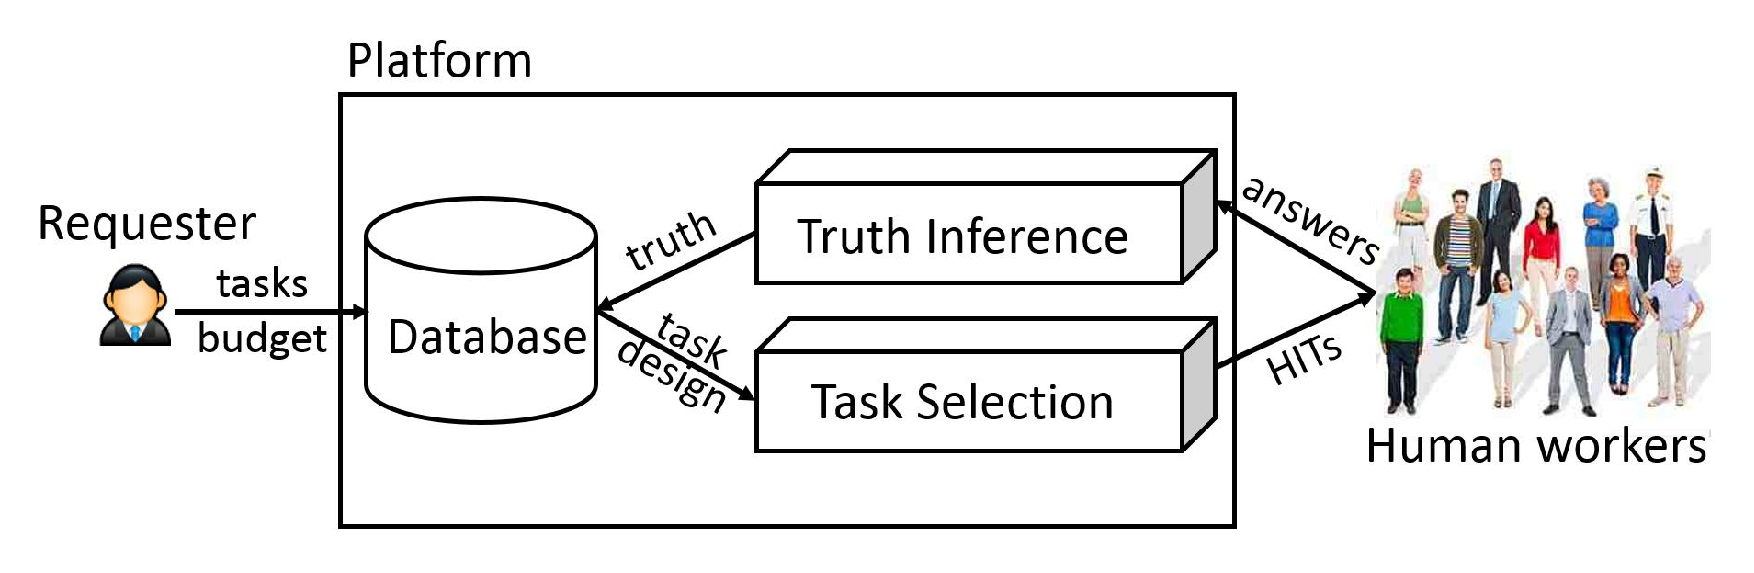
\includegraphics[width=0.8\textwidth]{submissions/yongxin/figs/task-select.pdf}
	\caption{An illustration of the workflow in task selection~\cite{DBLP:journals/tkde/LiWZF16}.}
	\label{fig:ts-flow}
\end{figure}

\fakeparagraph{Task Selection}
In this stage, human workers can freely choose the desired HITs and an HIT is assigned to the first worker who picks it.
This mode is also known as \textit{worker selected tasks (WST)} mode in the early studies~\cite{DBLP:conf/gis/KazemiS12,DBLP:conf/gis/DengSD13}.
To attract the human workers, existing studies usually focus on \textit{task design} in this type of interaction.
Specifically, \cite{DBLP:journals/tkde/LiWZF16,sigmod17tutorial} introduce \textit{task types} and \textit{task settings} as the fundamental problems in the task design.
When designing the task types, the crowdsourcing platforms need to carefully choose the format of the tasks.
For example, a problem with single choice is usually easier to be answer by the workers than the problem with multiple choices.
As a result, more studies focus on the tasks with single choice (\eg ~\cite{DBLP:journals/pvldb/FirmaniSS16,DBLP:conf/sigmod/WangLKFF13,DBLP:conf/icde/ZengTCZ18}) than the tasks with multiple choices (\eg \cite{DBLP:journals/pvldb/WangKFF12}).
However, the tasks with multiple choices are relatively more profitable for the workers and more helpful for inferring the truth (\ie the second stage).
A good task design combines these two types in practice.
For instance, Vasilis \etal~\cite{DBLP:conf/sigmod/VerroiosGP17} propose the approach called Waldo
to detect the difficult tasks with multiple choices and only resolve them by single choice.
When considering the task settings, the crowdsourcing platforms mainly determine the \textit{pricing} and \textit{timing} of the tasks.
Usually, a high price can intuitively attract more workers, thereby reducing the total time to complete a task (\ie low latency). 
However, a high price does not always indicate a good quality of the answer~\cite{DBLP:conf/aaai/FaradaniHI11}.
Therefore, a good task design needs to consider the trade-off between the pricing and timing.
For instance, Yihan \etal \cite{DBLP:journals/pvldb/GaoP14} applies Markov Decision Process to determine the price and deadline of the tasks.
Vasilis \etal \cite{DBLP:conf/sigmod/VerroiosLG15} designs a dynamic-programming based method in the task setting while simultaneously choosing the proper task type.

\fakeparagraph{Truth Inference}
In this stage, the crowdsourcing platform will collect the answers from the workers after they accomplish their selected tasks.
The challenge in this stage is how to infer the truth of each task based on the different tasks' answers collected from human workers~\cite{sigmod17tutorial}. 
Many solutions have been proposed to solve the problem of truth inference.
A simple solution is to use majority voting, where the truth is viewed as the majority answer of the workers.
However, this method overlooks the fact that the workers usually have different qualities in practice.
To obtain the worker's quality, one way is to use the hidden test, where a golden question is injected in an HIT.
Since the platform knows the truth of this golden question, it can estimate the workers' quality more accurately.
However, the hidden test takes more money since the workers need to complete these extra tasks.
Moreover, as reported in~\cite{DBLP:journals/pvldb/ZhengLLSC17}, the hidden tests may not improve much quality. 
Therefore, existing studies usually focus on inferring the truth without the hidden tests.
The most classic framework is Expectation Maximization (EM)~.
The EM method is firstly proposed in \cite{dempster1977maximum},
which leverages all the collected answers from the workers,
and updates each worker's quality and each task's true answer until convergence~\cite{DBLP:journals/tkde/LiWZF16}.
Other studies use the Graph-based methods~\cite{zhao2015crowd,karger2011iterative},
where a worker's quality is represented as a node
and is derived by the graphical model inference~\cite{koller2009probabilistic}.

\subsection{Task Recommendation By Platforms}\label{sec:ta-recommend}
There are many crowdsourcing platforms which take another mode \ie task recommendation by platforms to interact with crowd workers during task assignment, such as Uber, Didi Chuxing \cite{add-Zeng1,add-Zeng2} and Facebook Editor.
Early studies formulate the task recommendation problem as bipartite graph matching problem. 
Specifically, workers and tasks can be represented by the vertices in the bipartite graph and the score to evaluate the suitability of a worker and a task can be denoted by the weight of the edges. 
Then the problem is to obtain an optimal matching in the bipartite graph.

\fakeparagraph{Statics Scenario}
When the information of tasks and workers is known in advance (or before task recommendation), exact algorithms (\eg Hungarian algorithm~) can optimally solve the problem.
Alternatively, Kazemi ~\etal \cite{DBLP:conf/gis/KazemiS12} reduce the bipartite graph into an instance of the \textit{maximum flow} problem~ and use the Ford-Fulkerson algorithm to obtain the exact result.
They also consider some practical issues.
For example, if for a task there are fewer workers who are suitable to perform it, the task should be recommended with higher priority.
The idea of entropy can be borrowed to represent this priority.
Another heuristic strategy is to iteratively assign the task to its most suitable workers.
To reduce the computation cost of exact solutions, various greedy based methods are proposed.
For example, \cite{to2016real} maximizes the total number of tasks which are accepted by the workers while considering a budget constraint.

\fakeparagraph{Dynamical Scenario}
In reality, the time when new tasks are submitted to the platform and the content of the tasks are unknown.
Besides, the workers also log in the platforms dynamically.
Thus, some studies address the task recommendation problem while considering the dynamics of tasks and workers.
They formulate the problem as online bipartite graph matching.
Karp \etal \cite{DBLP:conf/stoc/KarpVV90} first propose the RANKING algorithm which yields a competitive ratio $1-1/e$ under the \textit{adversarial order model} and the ratio is proven to be the lower bound of any online algorithm.
%{GREEDY} recommends a new task to an arbitrarily chosen available worker.
%RANDOM differs in that the worker is uniformly sampled.
%The competitive ratios of {GREEDY} and RANDOM are both 0.5 under the \textit{adversarial order model}.
%RANKING is a two-phase algorithm.
%In the first phase, a random permutation of workers is picked and it represents the priority (\ie rank) of the workers.
%In the second phase, a {newly appeared} task will be recommended to the available worker with the highest rank.
%RANKING yields a competitive ratio $1-1/e$ under the \textit{adversarial order model}.
In~\cite{DBLP:conf/icde/TongSDWC16}, Tong \etal borrow the idea of secretary problem and devise a two-phase based framework.
%In the first half of vertices, {GREEDY} is used to determine the final recommendation.
%In the other half of vertices, they first find a global matching and then determine the final recommendation based on the global matching.
Their proposed algorithms achieve competitive ratios of 0.25 and 0.125 under the \textit{random order model}.
In \cite{add-VLDB16}, an comprehensive experimental study has been made and the greedy algorithm is proved to be competitive in real scenarios.
More flexible and adaptive online matching algorithms have also been proposed in \cite{add-ICDE17, add-VLDB17, add-DASFAA18, add-ICDE19}. 
In addition, Zhang \etal \cite{DBLP:conf/kdd/ZhangHMWZFGY17} focus on predicting the acceptance ratio of workers in task recommendation via machine learning techniques.
They treat the rejected tasks by workers as new tasks that can be re-recommended to other workers.
We refer readers to the comprehensive surveys~\cite{add-VLDBJ} for more details on task assignment approaches.

\section{Human-Human Interaction: Incentive Mechanism}
\label{sec:human-human}
Despite the essential interactions between humans and platforms, the sociality from humans has made human-human interactions more and more important in the future of work.
These interactions, which we summarize as the incentive mechanisms, depict how workers interact with each other and focus on how to design mechanisms to motivate workers.
To be more specific, on one hand, workers tend to be multi-skilled and social as crowdsourcing develops.
Those positive interactions (\eg complementary in skills or closeness in social contact) between humans can help improve the satisfaction of the workers and performance of the platforms.
On the other hand, the freewill of humans enables selfish workers.
Those malicious factors lead to inevitable competition, which needs to be treated carefully.
Correspondingly, we categorize the human-human interactions as collaborative interaction and competitive interaction.
In the following of this section, we will discuss about them respectively.

\subsection{Collaborative Interaction}
\label{subsec:hh-coll}
An important kind of human-human interaction is the collaborative interaction.
On one hand, tasks become more and more complicated and they usually require multiple skills to accomplish.
Workers with different skills should collaborate to accomplish the complicated tasks.
On the other hand, social factor may be helpful to improve the task quality and latency.
For example, two workers which are good friends may accomplish the tasks with higher quality and lower latency.
In a word, in this part we introduce two representative collaborative factors in human-human interaction, \ie multi-skill factor and social factor.

\fakeparagraph{Multi-skill Factor}
Multi-skill factor is one of the significant factors to depict complicated tasks and has been widely studied in recent years.
In early studies like \cite{aaai12taskassignment,icml13adaptive}, the skills are formulated as the skill level value representing the probability that a worker submits the true answer.
\cite{kdd13transfer} utilizes the formulation of expertise level and applies a transfer learning model to estimate the expertise levels in all categories.
To overcome the disadvantage that a single value cannot depict multiple skills, \cite{edbt15crowdsel} extends the formulation to the environment of multiple skills and uses a vector called latent skill category to represent how a worker is familiar with different skills.
\cite{dse17topk} and \cite{aamas16truthful} study the so-called team formation problem and propose the solutions with the help of social networks and road networks, respectively.
In the future of work, despite of existing formulations like skill level and team formation, we may facet a more complicated multi-skill situation where the task requires a time dependency of skills.
Under this situation, a task may require a worker with skill $A$ and a worker with skill $B$ sequentially, which requires a novel solution based on the accurate estimation of worker skills.



\fakeparagraph{Social Factor}
As human workers have their own social roles apart from workers on crowdsourcing platforms, the social factor can also influence the completion of tasks.
Some work has used the social factors like relationships on social networks and communities \cite{add-CIKM19} to help increase the crowdsourcing quality.
In \cite{DBLP:journals/pvldb/CaoSTC12}, the authors address the decision making question answering by crowdsourcing on micro-blog services. 
One of the most fundamental steps in addressing the problem is to estimate the rating score of different workers.
The authors first construct a user-graph with Twitter data according to the workers' forwarding operation retweet, and then rank the users in the constructed graph.
Therefore, expertises that are frequently followed by other twitters can be found through the user graph easily.
In \cite{www14community}, the authors propose a novel community-based Bayesian label aggregation model, which can predict the labels of different workers by assuming that each worker belongs to a certain community.
Some other work models the social relationships with game theory and reveals the importance of social factors in crowdsourcing.
In \cite{tmc19strategic}, it considers the social team formation problem in crowdsourcing, where a team of socially connected professional workers can work together collaboratively.
It focuses on designing truthful mechanisms according to workers’ social structure, skill, and working cost to guarantee that a worker’s utility is optimized when he behaves honestly. 
\cite{TIST17} directly studies the social factors in incentive mechanisms in crowdsourcing and finds that collaboration leads to better accuracy and more outputs.
It reveals that in pair-work crowdsourcing, when one of the workers tries to exit the task, the partner is very likely to make him/her stay for higher payment and for enjoying the tasks together.
Therefore, social furtherance incentives can create a win-win scenario for both the platform and the human workers.

%%%%%%%%%%
% delte from here if space is limited
\tabref{tab:h-h-col} summarizes existing works on collaborative interactions.
We summarize that both multi-skill and social factors raise attention but their formulation needs to be further completed to suit for more challenging situations.
\begin{table}[t]
	\centering
	\caption{Related works on collaborative interaction.}\label{tab:h-h-col}
	\setlength{\tabcolsep}{1.5mm}{
		\begin{tabular}{|c|c|c|c|}
			\hline
			Reference & Interaction & Factor &  Formulation  \\ \hline
			\cite{aaai12taskassignment} & Collaborative & Multi-Skill Factor & Skill Level \\ \hline
			\cite{icml13adaptive} & Collaborative & Multi-Skill Factor & Skill Level \\ \hline
            \cite{kdd13transfer} & Collaborative & Multi-Skill Factor & Expertise Level \\ \hline
            \cite{edbt15crowdsel} & Collaborative & Multi-Skill Factor & Latent Skill Category \\ \hline
            \cite{dse17topk} & Collaborative & Multi-Skill Factor & Team Formulation \\ \hline
            \cite{aamas16truthful} & Collaborative & Multi-Skill Factor & Team Formulation \\ \hline
            \cite{DBLP:journals/pvldb/CaoSTC12} & Collaborative & Social Factor & Rating Score \\ \hline
            \cite{www14community} &Collaborative & Social Factor & Label Prediction \\ \hline
            \cite{tmc19strategic} &Collaborative & Social Factor & Team Formulation \\ \hline
             \cite{TIST17} & Collaborative& Social Factor & Social Furtherance \\ \hline
		\end{tabular}
	}
\end{table}
%%% delte end

\subsection{Competitive Interaction}
\label{subsec:hh-comp}

Despite the collaboration in human-human interaction, there also exists competitions in the interaction of crowdsourcing.
Different from collaboration, malicious competitions may reduce the quality of the tasks or even destroy the human-in-the-loop ecosystem.
However, passive competitions can be beneficial if treated carefully.
In this part we envision how to utilize competitions to encourage workers to participate in completing tasks with higher quality and lower latency.
In details, depending on whether the reward is monetary or immaterial, we categorize the interaction as monetary factor and non-monetary factor.

\fakeparagraph{Monetary Factor}
Monetary is one of the most important factors that can influence how workers perform.
Current studies usually formulate the monetary factor in competitive human-human interaction based on the game theory.
In a word, a carefully designed pricing mechanism should be able to provide a well balance between payments (\eg prices paid to workers) and to promote workers to submit the truthful information. 
Most works provide auction-based solutions to model the competitive interaction between humans.
Workers need to bid their expected prices to the platform, and the platform chooses workers to accomplish tasks based on the proposed mechanisms.
Notice that even there is no direct communication among workers, the mechanism which is known by all workers in fact provides an indirect competitive interaction among workers.
Because of the selfishness of workers, the mechanisms should be truthful, \ie the mechanism guarantees that workers cannot obtain more reward if they provide  false information.
Besides, another consideration of designing the mechanism is how to balance various constraints and objectives.
For example, \cite{www13truthful,focs14mechanism,add-SIGMOD18} aim at maximizing the utility (\ie the value obtained from the workers) while making sure that the total budget is under a given threshold.
Different from \cite{www13truthful} and \cite{focs14mechanism}, \cite{www13pricing} focuses on two different objectives: maximizing the number of accomplished tasks with constrained budget and minimizing total payment with least number of accomplished tasks.
In future of work, the interaction may facet more challenging situations.
Firstly, the private information may be more complicated (comparing with current research where each worker is associated with a private expected value).
For example, each worker may privately possess the total order of preference to the tasks, the capability of different kinds of tasks, \etc.
Besides, in future of work there can be other practical trade-offs and objectives like trade-off between payment and quality of tasks or between payment and latency of workers.
These complicated private information and various objectives can raise more challenging problems in the competitive human-human interaction.

\fakeparagraph{Non-Monetary Factor}
Despite the dominant role of the monetary factor, none-monetary factor (\eg gamification, volunteering \etc) also plays an important role in the competitive human-human interaction.
Specifically, gamification can attract workers to join the procedure \cite{sigir12game} and result in positive competitions that motivate workers to provide better services \cite{cikm14game}.
For example, \cite{sigir12game} develops a series of games to attract workers to attain the crowdsourcing tasks.
Further experiments show that the proposed games can improve the quality and latency of the accomplished tasks.
Compared with \cite{sigir12game}, \cite{cikm14game} combines the luck games (\eg lottery) with crowdsourcing.
Each worker is given one or more lotteries and which worker can be paid is related not only to the quality of the accomplished tasks, but also to the lottery results.
In the future of work, non-monetary factor may become more and more important.
An interesting study direction is to formally model how non-monetary factor like gamification produce positive competitive interaction and impact the performance of workers in crowdsourcing.
%%%%%%%%%%
% delte from here if space is limited

\tabref{tab:h-h-com} summarizes existing works on competitive interactions.
We summarize that most existing works focus on the interaction with monetary factor.
Non-Monetary factor, although lacking in systematic study in crowdsourcing, can also play an important role in future work.
\begin{table}[t]
	\centering
	\caption{Related works on competitive interaction.}\label{tab:h-h-com}
	\setlength{\tabcolsep}{1.5mm}{
		\begin{tabular}{|c|c|c|c|}
			\hline
			Reference & Interaction & Factor &  Formulation  \\ \hline
			\cite{www13pricing} & Competitive & Monetory Factor & Auction \\ \hline
			\cite{www13truthful} & Competitive & Monetory Factor & Auction \\ \hline
			\cite{focs14mechanism} & Competitive & Monetory Factor & Auction \\ \hline
			\cite{is19competitivecs} & Competitive & Monetory Factor & Collaboration \\ \hline
			\cite{sigir12game} & Competitive & Non-Monetory Factor & Relevance Assessments \\ \hline
			\cite{cikm14game} & Competitive & Non-Monetory Factor & Lottory \\ \hline
		\end{tabular}
	}
\end{table}
%%% delte end

\section{Future Direction: Cross-Platform Interaction}

In the previous sections, we have discussed about human-platform and human-human interaction in existing crowdsourcing platforms.
In this section, we are going to introduce a future direction: the cross-platform interaction.
Nowadays, there is a large amount of commercial crowdsourcing platforms that divide the online job markets into many pieces.
If these platforms can work together as a federation (as illustrated in \figref{fig:federation}), task requesters will have a higher chance to meet more professional workers and workers will also have more career opportunities.
However, sensitive information like worker profiles, professional skills and working histories cannot be shared freely between different platforms, for the purpose of preserving each human worker's privacy.
Therefore, the cross-platform interaction should be more carefully designed and the major concern is how to preserve the privacy of human workers from different platforms.

There is rich literature on privacy-preserving schemes, including encryption methods like homomorphic encryption \cite{FHE} and randomized algorithms like differential privacy \cite{ICALP06}.
%The propositions of privacy-preserving frameworks for basic operations like gradient descent \cite{CCS16} and frequency estimation \cite{NIPS14} also make it possible to design secure protocols for more complicated functions and systems like interactive modules in the federation of crowdsourcing platforms. 
Next, we will discuss about the possible shape of the interactive modules including cross-platform task assignment and cross-platform incentive mechanism, as well as the privacy-preserving techniques behind them.

\begin{figure}
	\centering
	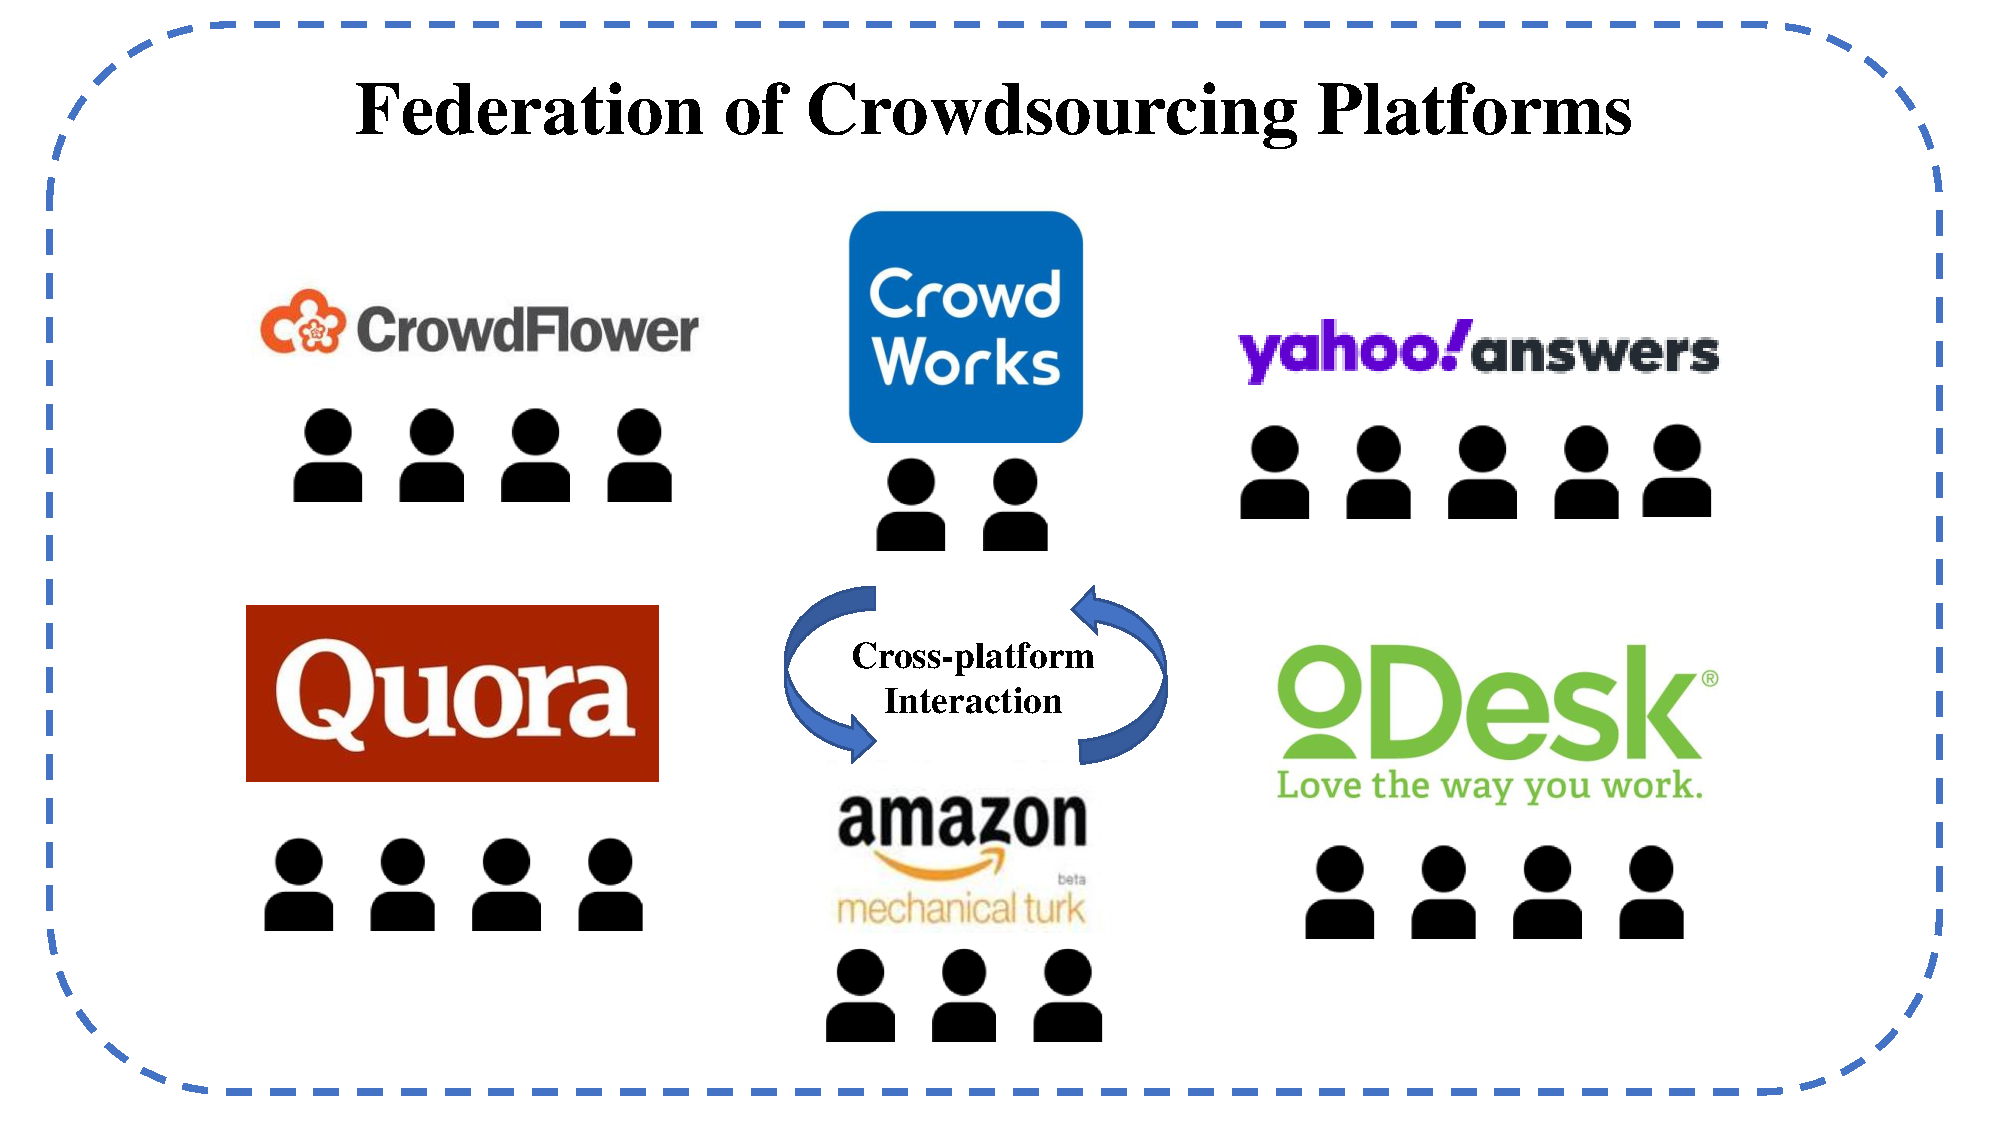
\includegraphics[scale=0.45]{submissions/yongxin/figs/federation.pdf}
	
	\caption{An illustration of the federation of crowdsourcing platforms}
	\label{fig:federation}
\end{figure}

\fakeparagraph{Cross-platform task assignment}
The interaction in cross-platform task assignment can be different from conventional task assignment where the platform has full knowledge of its tasks and workers.
In a cross-platform task assignment scenario, workers will have opportunity to complete the tasks from other platforms.
We conceive two types of interaction in cross-platform task assignment: interaction by recommendation and by negotiation.
In the first type, surplus tasks on each platform can be shared with other platforms in the form of recommendation and the task specifications and the original links will be given.
The recommended tasks from other platforms will be visible in the task pool of each platform, and the workers can select the preferred tasks freely.
If they are interested in tasks from other platforms, they can have a quick registration through the link and become a cross-platform worker.
Considering that there might be a huge number of pending tasks in the whole platform federation, one of the major challenge is to recommend for each worker a personalized ranking list of tasks so that they can locate their favorite tasks in a short time.
A federated recommender system can be designed to protect the privacy of each worker while making personalized and accurate recommendations.
Randomized algorithms like locality-sensitive hashing are possible solutions to protect private tags of workers in federated recommender systems. 
In the second type, the platforms will negotiate with each other at first.
For example, there are surplus tasks on Figure Eight and the platform would like to borrow workers from AMT to finish these tasks. 
Figure Eight will negotiate with AMT, about the amount and types of the tasks and the profit shares meanwhile AMT can provide some information on workers to select appropriate tasks.
Afterwards, the selected tasks will become available to workers on AMT as new tasks.
After the completion of tasks, AMT will return only the results and Figure Eight should know little about the specific workers who complete them.
To protect the private profiles and working histories of the workers, there should be anonymization techniques during the negotiation.
For example, AMT can only provide the summary or aggregated results of worker abilities for Figure Eight to decide which tasks can be shared.
Another possible problem is that AMT can hide the information of profit shares from the workers if the payment by Figure Eight is much higher and how to ensure the trust and fairness remains challenging. 

\fakeparagraph{Cross-platform incentive mechanism}
Similar to cross-platform task assignment, cross-platform incentive mechanism also faces privacy challenges.
We mainly focus on incentive mechanisms in collaborative scenarios, where the privacy leakage is much more likely to happen.
In a collaborative scenario, workers from different platforms can have a chance to form groups to perform cross-platform tasks.
In one way, they can cooperate to perform a batch of simple tasks respectively and aggregate the results afterwards.
For example, the federated platform publishes a task of labeling a large number of CT images.
Expertises like doctors from different platforms can form a team to accomplish the tasks.
They can divide the tasks according to their areas of expertise so the group work can be more efficient. 
In another way, each worker can also perform one or several steps in the working pipeline of complicated tasks.
For example, the task is to tag all the objects in photos of street views and then to annotate the texts on street signs and buildings.
It can be divided into several steps, including marking all the objects, annotating the texts and double-checking the results, where each step can be conducted by workers from different platforms.
In both ways, the federated platform should design team formation algorithms based on social networks or ability tags of different workers, which also has risk of privacy leakage.
Although there is plenty of work concerning privacy issues in social networks, how to preserve personal information while finding like-minded partners still remains a challenge. 

\section{Conclusion}
Crowdsourcing has attracted much popularity in recent years, due to its high efficiency in dealing with computer-hard tasks by human workers.
However, we have noticed the problem that humans are often treated as machines.
To deal with such problem, managing the interaction among the workers and platforms is essential.
In this paper, we categorize and analyze different interactions on crowdsourcing platforms, and discuss about the challenges and existing work on human-platform interaction and human-human interaction respectively.
Finally, we envision a new type of interaction, the cross-platform interaction. 
We hope in the future of crowdsourcing, there will be a federation of platforms that offer much more opportunities to everyone everywhere and human workers will be treated as fully human with respect and dignity.

\bibliographystyle{IEEEtran}

\begin{thebibliography}{10}
	\providecommand{\url}[1]{#1}
	\csname url@samestyle\endcsname
	\providecommand{\newblock}{\relax}
	\providecommand{\bibinfo}[2]{#2}
	\providecommand{\BIBentrySTDinterwordspacing}{\spaceskip=0pt\relax}
	\providecommand{\BIBentryALTinterwordstretchfactor}{4}
	\providecommand{\BIBentryALTinterwordspacing}{\spaceskip=\fontdimen2\font plus
		\BIBentryALTinterwordstretchfactor\fontdimen3\font minus
		\fontdimen4\font\relax}
	\providecommand{\BIBforeignlanguage}[2]{{%
			\expandafter\ifx\csname l@#1\endcsname\relax
			\typeout{** WARNING: IEEEtran.bst: No hyphenation pattern has been}%
			\typeout{** loaded for the language `#1'. Using the pattern for}%
			\typeout{** the default language instead.}%
			\else
			\language=\csname l@#1\endcsname
			\fi
			#2}}
	\providecommand{\BIBdecl}{\relax}
	\BIBdecl
	
	\bibitem{DBLP:journals/tkde/TongCZJSL18}
	Y.~Tong, L.~Chen, Z.~Zhou, H.~V. Jagadish, L.~Shou, and W.~Lv, ``{SLADE:} {A}
	smart large-scale task decomposer in crowdsourcing,'' \emph{{IEEE} TKDE},
	vol.~30, no.~8, pp. 1588--1601, 2018.
	
	\bibitem{DBLP:journals/tkde/LiWZF16}
	G.~Li, J.~Wang, Y.~Zheng, and M.~J. Franklin, ``Crowdsourced data management:
	{A} survey,'' \emph{{IEEE} TKDE}, vol.~28, no.~9, pp. 2296--2319, 2016.
	
	\bibitem{DBLP:conf/gis/KazemiS12}
	L.~Kazemi and C.~Shahabi, ``Geocrowd: enabling query answering with spatial
	crowdsourcing,'' in \emph{GIS}, 2012, pp. 189--198.
	
	\bibitem{DBLP:conf/gis/DengSD13}
	D.~Deng, C.~Shahabi, and U.~Demiryurek, ``Maximizing the number of worker's
	self-selected tasks in spatial crowdsourcing,'' in \emph{GIS}, 2013, pp.
	314--323.
	
	\bibitem{sigmod17tutorial}
	G.~Li, Y.~Zheng, J.~Fan, J.~Wang, and R.~Cheng, ``Crowdsourced data management:
	Overview and challenges,'' in \emph{SIGMOD}, 2017, pp. 1711--1716.
	
	\bibitem{DBLP:journals/pvldb/FirmaniSS16}
	D.~Firmani, B.~Saha, and D.~Srivastava, ``Online entity resolution using an
	oracle,'' \emph{{PVLDB}}, vol.~9, no.~5, pp. 384--395, 2016.
	
	\bibitem{DBLP:conf/sigmod/WangLKFF13}
	J.~Wang, G.~Li, T.~Kraska, M.~J. Franklin, and J.~Feng, ``Leveraging transitive
	relations for crowdsourced joins,'' in \emph{{SIGMOD}}, 2013, pp. 229--240.
	
	\bibitem{DBLP:conf/icde/ZengTCZ18}
	Y.~Zeng, Y.~Tong, L.~Chen, and Z.~Zhou, ``Latency-oriented task completion via
	spatial crowdsourcing,'' in \emph{ICDE}, 2018, pp. 317--328.
	
	\bibitem{DBLP:journals/pvldb/WangKFF12}
	J.~Wang, T.~Kraska, M.~J. Franklin, and J.~Feng, ``Crowder: Crowdsourcing
	entity resolution,'' \emph{{PVLDB}}, vol.~5, no.~11, pp. 1483--1494, 2012.
	
	\bibitem{DBLP:conf/sigmod/VerroiosGP17}
	V.~Verroios, H.~Garcia{-}Molina, and Y.~Papakonstantinou, ``Waldo: An adaptive
	human interface for crowd entity resolution,'' in \emph{{SIGMOD}}, 2017, pp.
	1133--1148.
	
	\bibitem{DBLP:conf/aaai/FaradaniHI11}
	S.~Faradani, B.~Hartmann, and P.~G. Ipeirotis, ``What's the right price?
	pricing tasks for finishing on time,'' in \emph{HCOMP}, 2011.
	
	\bibitem{DBLP:journals/pvldb/GaoP14}
	Y.~Gao and A.~G. Parameswaran, ``Finish them!: Pricing algorithms for human
	computation,'' \emph{{PVLDB}}, vol.~7, no.~14, pp. 1965--1976, 2014.
	
	\bibitem{DBLP:conf/sigmod/VerroiosLG15}
	V.~Verroios, P.~Lofgren, and H.~Garcia{-}Molina, ``tdp: An optimal-latency
	budget allocation strategy for crowdsourced {MAXIMUM} operations,'' in
	\emph{{SIGMOD}}, 2015, pp. 1047--1062.
	
	\bibitem{DBLP:journals/pvldb/ZhengLLSC17}
	Y.~Zheng, G.~Li, Y.~Li, C.~Shan, and R.~Cheng, ``Truth inference in
	crowdsourcing: Is the problem solved?'' \emph{PVLDB}, vol.~10, no.~5, pp.
	541--552, 2017.
	
	\bibitem{dempster1977maximum}
	A.~P. Dempster, N.~M. Laird, and D.~B. Rubin, ``Maximum likelihood from
	incomplete data via the em algorithm,'' \emph{Journal of the Royal
		Statistical Society}, vol.~39, no.~1, pp. 1--22, 1977.
	
	\bibitem{zhao2015crowd}
	Z.~Zhao, F.~Wei, M.~Zhou, W.~Chen, and W.~Ng, ``Crowd-selection query
	processing in crowdsourcing databases: A task-driven approach.'' in
	\emph{EDBT}, 2015, pp. 397--408.
	
	\bibitem{karger2011iterative}
	D.~R. Karger, S.~Oh, and D.~Shah, ``Iterative learning for reliable
	crowdsourcing systems,'' in \emph{NIPS}, 2011, pp. 1953--1961.
	
	\bibitem{koller2009probabilistic}
	D.~Koller and N.~Friedman, \emph{Probabilistic graphical models: principles and
		techniques}.\hskip 1em plus 0.5em minus 0.4em\relax MIT press, 2009.
	
	\bibitem{add-Zeng1}
	Y.~Tong, Y.~Zeng, Z.~Zhou, L.~Chen, J.~Ye, and K.~Xu, ``A unified approach to
	route planning for shared mobility,'' \emph{{PVLDB}}, vol.~11, no.~11, pp.
	1633--1646, 2018.
	
	\bibitem{add-Zeng2}
	Y.~Zeng, Y.~Tong, and L.~Chen, ``Last-mile delivery made practical: An
	efficient route planning framework with theoretical guarantees,''
	\emph{{PVLDB}}, vol.~13, no.~3, pp. 320--333, 2019.
	
	\bibitem{to2016real}
	H.~To, L.~Fan, L.~Tran, and C.~Shahabi, ``Real-time task assignment in
	hyperlocal spatial crowdsourcing under budget constraints,'' in
	\emph{PerCom}, 2016, pp. 1--8.
	
	\bibitem{DBLP:conf/stoc/KarpVV90}
	R.~M. Karp, U.~V. Vazirani, and V.~V. Vazirani, ``An optimal algorithm for
	on-line bipartite matching,'' in \emph{STOC}, 1990, pp. 352--358.
	
	\bibitem{DBLP:conf/icde/TongSDWC16}
	Y.~Tong, J.~She, B.~Ding, L.~Wang, and L.~Chen, ``Online mobile micro-task
	allocation in spatial crowdsourcing,'' in \emph{ICDE}, 2016, pp. 49--60.
	
	\bibitem{add-VLDB16}
	Y.~Tong, J.~She, B.~Ding, L.~Chen, T.~Wo, and K.~Xu, ``Online minimum matching
	in real-time spatial data: Experiments and analysis,'' \emph{{PVLDB}},
	vol.~9, no.~12, pp. 1053--1064, 2016.
	
	\bibitem{add-ICDE17}
	T.~Song, Y.~Tong, L.~Wang, J.~She, B.~Yao, L.~Chen, and K.~Xu, ``Trichromatic
	online matching in real-time spatial crowdsourcing,'' in \emph{ICDE}, 2017,
	pp. 1009--1020.
	
	\bibitem{add-VLDB17}
	Y.~Tong, L.~Wang, Z.~Zhou, B.~Ding, L.~Chen, J.~Ye, and K.~Xu, ``Flexible
	online task assignment in real-time spatial data,'' \emph{{PVLDB}}, vol.~10,
	no.~11, pp. 1334--1345, 2017.
	
	\bibitem{add-DASFAA18}
	Q.~Tao, Y.~Zeng, Z.~Zhou, Y.~Tong, L.~Chen, and K.~Xu, ``Multi-worker-aware
	task planning in real-time spatial crowdsourcing,'' in \emph{DASFAA}, 2018,
	pp. 301--317.
	
	\bibitem{add-ICDE19}
	Y.~Wang, Y.~Tong, C.~Long, P.~Xu, K.~Xu, and W.~Lv, ``Adaptive dynamic
	bipartite graph matching: {A} reinforcement learning approach,'' in
	\emph{ICDE}, 2019, pp. 1478--1489.
	
	\bibitem{DBLP:conf/kdd/ZhangHMWZFGY17}
	L.~Zhang, T.~Hu, Y.~Min, G.~Wu, J.~Zhang, P.~Feng, P.~Gong, and J.~Ye, ``A taxi
	order dispatch model based on combinatorial optimization,'' in \emph{KDD},
	2017, pp. 2151--2159.
	
	\bibitem{add-VLDBJ}
	\BIBentryALTinterwordspacing
	Y.~Tong, Z.~Zhou, Y.~Zeng, L.~Chen, and C.~Shahabi, ``Spatial crowdsourcing: a
	survey,'' \emph{The VLDB Journal}, 2019. [Online]. Available:
	\url{https://doi.org/10.1007/s00778-019-00568-7}
	\BIBentrySTDinterwordspacing
	
	\bibitem{aaai12taskassignment}
	C.~Ho and J.~W. Vaughan, ``Online task assignment in crowdsourcing markets,''
	in \emph{{AAAI}}, 2012.
	
	\bibitem{icml13adaptive}
	C.~Ho, S.~Jabbari, and J.~W. Vaughan, ``Adaptive task assignment for
	crowdsourced classification,'' in \emph{{ICML}}, 2013, pp. 534--542.
	
	\bibitem{kdd13transfer}
	Z.~Zhao, D.~Yan, W.~Ng, and S.~Gao, ``A transfer learning based framework of
	crowd-selection on twitter,'' in \emph{{KDD}}, 2013, pp. 1514--1517.
	
	\bibitem{edbt15crowdsel}
	Z.~Zhao, F.~Wei, M.~Zhou, W.~Chen, and W.~Ng, ``Crowd-selection query
	processing in crowdsourcing databases: {A} task-driven approach,'' in
	\emph{{EDBT}}, 2015, pp. 397--408.
	
	\bibitem{dse17topk}
	D.~Gao, Y.~Tong, J.~She, T.~Song, L.~Chen, and K.~Xu, ``Top-k team
	recommendation and its variants in spatial crowdsourcing,'' \emph{Data
		Science and Engineering}, vol.~2, no.~2, pp. 136--150, 2017.
	
	\bibitem{aamas16truthful}
	W.~Wang, Z.~He, P.~Shi, W.~Wu, and Y.~Jiang, ``Truthful team formation for
	crowdsourcing in social networks: (extended abstract),'' in \emph{AAMAS},
	2016, pp. 1327--1328.
	
	\bibitem{add-CIKM19}
	L.~Zhang, T.~Song, Y.~Tong, Z.~Zhou, D.~Li, W.~Ai, L.~Zhang, G.~Wu, Y.~Liu, and
	J.~Ye, ``Recommendation-based team formation for on-demand taxi-calling
	platforms,'' in \emph{CIKM}, 2019, pp. 59--68.
	
	\bibitem{DBLP:journals/pvldb/CaoSTC12}
	C.~C. Cao, J.~She, Y.~Tong, and L.~Chen, ``Whom to ask? jury selection for
	decision making tasks on micro-blog services,'' \emph{PVLDB}, vol.~5, no.~11,
	pp. 1495--1506, 2012.
	
	\bibitem{www14community}
	M.~Venanzi, J.~Guiver, G.~Kazai, P.~Kohli, and M.~Shokouhi, ``Community-based
	bayesian aggregation models for crowdsourcing,'' in \emph{{WWW}}, 2014, pp.
	155--164.
	
	\bibitem{tmc19strategic}
	W.~Wang, Z.~He, P.~Shi, W.~Wu, Y.~Jiang, B.~An, Z.~Hao, and B.~Chen,
	``Strategic social team crowdsourcing: Forming a team of truthful workers for
	crowdsourcing in social networks,'' \emph{{IEEE} TMC}, vol.~18, no.~6, pp.
	1419--1432, 2019.
	
	\bibitem{TIST17}
	O.~Feyisetan and E.~Simperl, ``Social incentives in paid collaborative
	crowdsourcing,'' \emph{{ACM} {TIST}}, vol.~8, no.~6, pp. 73:1--73:31, 2017.
	
	\bibitem{www13truthful}
	A.~Singla and A.~Krause, ``Truthful incentives in crowdsourcing tasks using
	regret minimization mechanisms,'' in \emph{{WWW}}, 2013, pp. 1167--1178.
	
	\bibitem{focs14mechanism}
	N.~Anari, G.~Goel, and A.~Nikzad, ``Mechanism design for crowdsourcing: An
	optimal 1-1/e competitive budget-feasible mechanism for large markets,'' in
	\emph{{FOCS}}, 2014, pp. 266--275.
	
	\bibitem{add-SIGMOD18}
	Y.~Tong, L.~Wang, Z.~Zhou, L.~Chen, B.~Du, and J.~Ye, ``Dynamic pricing in
	spatial crowdsourcing: {A} matching-based approach,'' in \emph{SIGMOD}, 2018,
	pp. 773--788.
	
	\bibitem{www13pricing}
	Y.~Singer and M.~Mittal, ``Pricing mechanisms for crowdsourcing markets,'' in
	\emph{{WWW}}, 2013, pp. 1157--1166.
	
	\bibitem{sigir12game}
	C.~Eickhoff, C.~G. Harris, A.~P. de~Vries, and P.~Srinivasan, ``Quality through
	flow and immersion: gamifying crowdsourced relevance assessments,'' in
	\emph{{SIGIR}}, 2012, pp. 871--880.
	
	\bibitem{cikm14game}
	M.~Rokicki, S.~Chelaru, S.~Zerr, and S.~Siersdorfer, ``Competitive game designs
	for improving the cost effectiveness of crowdsourcing,'' in \emph{{CIKM}},
	2014, pp. 1469--1478.
	
	\bibitem{is19competitivecs}
	S.~K. Mridha and M.~Bhattacharyya, ``Introducing collaboration in competitive
	crowdsourcing markets,'' \emph{{IEEE} Intelligent Systems}, vol.~34, no.~1,
	pp. 23--31, 2019.
	
	\bibitem{FHE}
	C.~Gentry, ``Fully homomorphic encryption using ideal lattices,'' in
	\emph{STOC}, 2009, pp. 169--178.
	
	\bibitem{ICALP06}
	C.~Dwork, ``Differential privacy,'' in \emph{ICALP}, 2006, pp. 1--12.
	
\end{thebibliography}


\end{document}
